% SPDX-FileCopyrightText: © 2021 Martin Michlmayr <tbm@cyrius.com>

% SPDX-License-Identifier: CC-BY-4.0

\documentclass[
	a4paper,
	fontsize=12pt,
	twoside=false,
	numbers=noenddot,
]{kaobook}

% Choose the language
\ifxetexorluatex
	\usepackage{polyglossia}
	\setmainlanguage{english}
\else
	\usepackage[english]{babel}
\fi

% Load the package for hyperreferences
\usepackage{kaorefs}

\renewcommand\labelitemi{\textbullet}% bullet

\hypersetup{
	colorlinks=true,
	linkcolor=blue,
	urlcolor=blue,
	pdfsubject={Primer on non-technical aspects of open-source projects and FOSS foundations},
	pdfkeywords={open source, free software, FOSS, foundations, sustainability, growth, success, digital infrastructure},
}

% License commands
\newcommand{\CCBY}[1]{\href{https://creativecommons.org/licenses/by/#1/}{CC BY #1}}
\newcommand{\CCBYSA}[1]{\href{https://creativecommons.org/licenses/by-sa/#1/}{CC BY-SA #1}}
\newcommand{\CCZERO}[1]{\href{https://creativecommons.org/publicdomain/zero/#1/}{CC0 #1}}
\newcommand{\CCPD}[1]{\href{https://creativecommons.org/publicdomain/mark/#1/}{public domain}}

%----------------------------------------------------------------------------------------

\begin{document}

\title{Growing Open-Source Projects with a Stable Foundation}

\author[Martin Michlmayr]{Martin Michlmayr}

\date{April 2021}

\frontmatter

\begin{titlepage}

\makeatletter
\begin{tikzpicture}[remember picture, overlay]
    \node (image) at (current page.center) [
	inner sep=0pt,
	outer sep=0pt,
	]{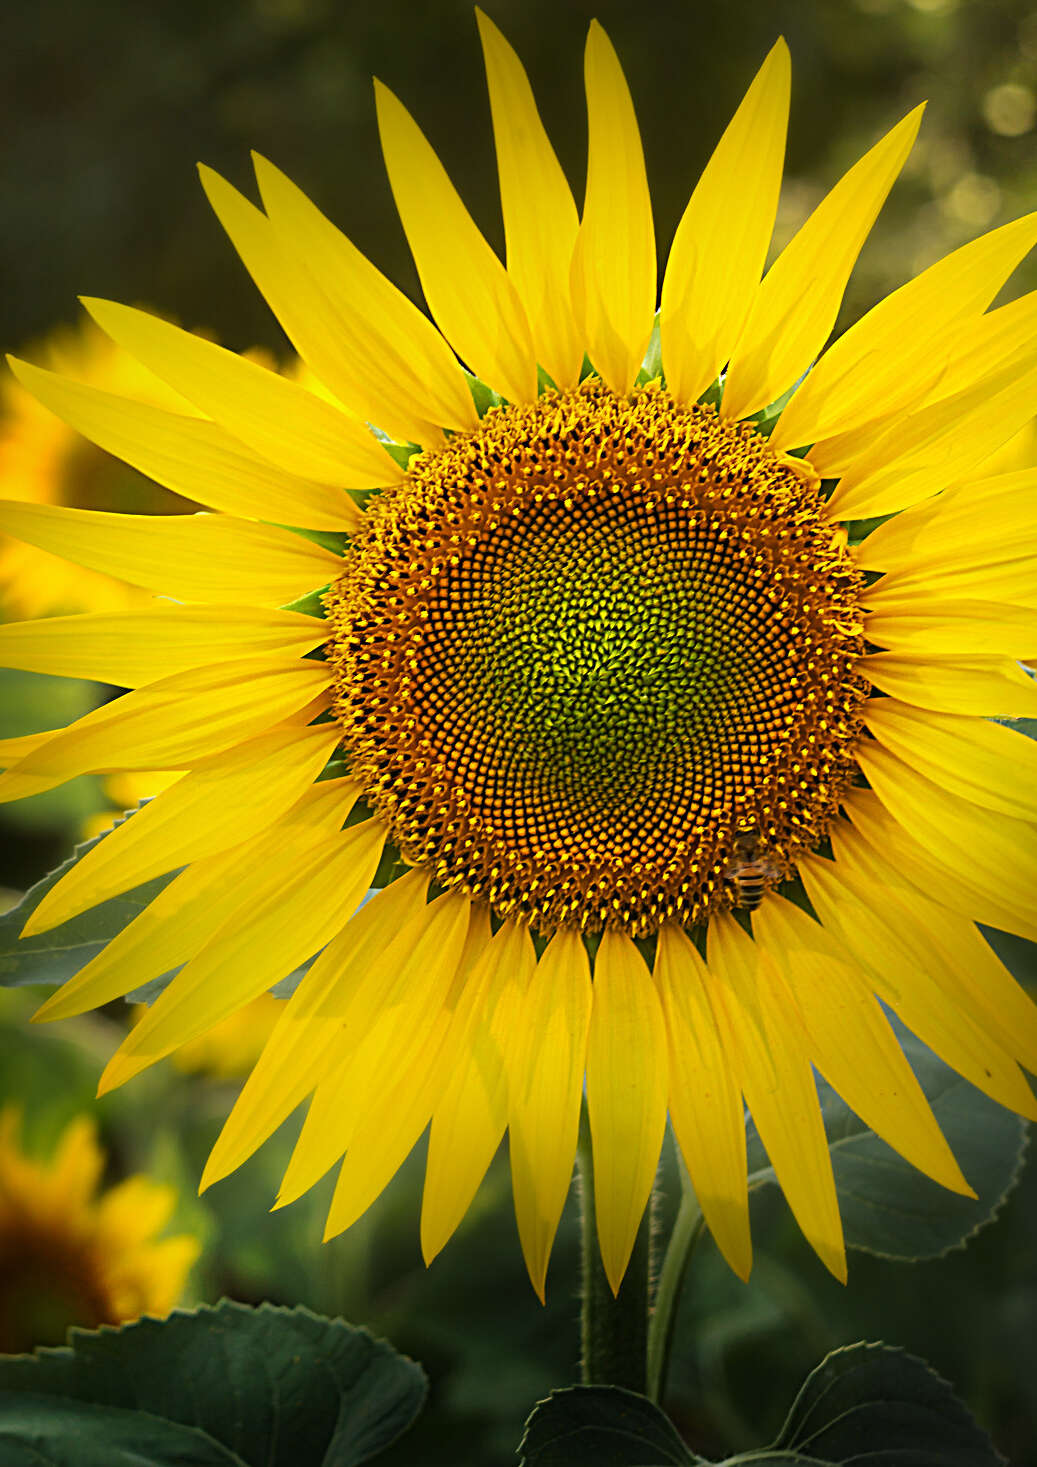
\includegraphics[width=\paperwidth,height=\paperheight,keepaspectratio=false]{images/comouflage}};
    \node [
	fill=gray!20!white,
	fill opacity=0.8,
	align=center,
	minimum width=\paperwidth,
	minimum height=2cm,
	anchor=north,
	inner ysep=1.2cm
    ] (Box1) at ([yshift=-21cm]current page.north) {
	{\Huge\textbf{Growing Open-Source Projects with a}}
	\\
	\\
	{\Huge\textbf{Stable Foundation}\par}
	\\
	\\
	\\
	{\LARGE \@author}
	\\
	\\
	\\
	{\Large \@date}
    };
\end{tikzpicture}
\makeatother

\end{titlepage}


% SPDX-FileCopyrightText: © 2021 Martin Michlmayr <tbm@cyrius.com>

% SPDX-License-Identifier: CC-BY-4.0

\chapter*{Preface}

Starting an open-source project is easy.  Running a successful project, on the other hand, comes with a lot of work and responsibilities, especially if the project attracts a large user base.

While open-source projects come in all shapes and forms, most projects encounter a similar set of growth issues throughout their life cycles.

This primer covers non-technical aspects that the majority of projects will have to consider at some point.  It also explains how FOSS foundations, non-profit organizations that support open-source projects, can help projects succeed and grow.

This primer explains:

\begin{itemize}

\item What issues and areas to consider

\item How other projects and foundations have approached these topics

\item What FOSS foundations bring to the table

\item How to choose a FOSS foundation

\end{itemize}


\index{preface}

\setchapterimage[9.5cm]{images/book}
\tableofcontents

%----------------------------------------------------------------------------------------

\mainmatter

% We don't use the margin feature of the kaobook class at all.
\pagelayout{wide}

\addpart{Background}


% SPDX-FileCopyrightText: © 2021 Martin Michlmayr <tbm@cyrius.com>

% SPDX-License-Identifier: CC-BY-4.0

\setchapterimage[9.5cm]{images/bridge}
\chapter{Open source as digital infrastructure}
\labch{digital-infrastructure}

Nadia Eghbal describes open source as digital infrastructure in her report \href{https://www.fordfoundation.org/work/learning/research-reports/roads-and-bridges-the-unseen-labor-behind-our-digital-infrastructure/}{Roads and Bridges}:

\begin{quote}

Much like roads or bridges, which anyone can walk or drive on, open source code can be used by anyone—from companies to individuals—to build software. This type of code makes up the digital infrastructure of our society today.

\end{quote}

Open source has fundamentally changed the way software is written.  Instead of starting a new software project entirely from scratch, programmers look for open source libraries that can be integrated to solve the problem at hand.  Furthermore, the advantages of open collaboration through open source is increasingly being recognized by companies, and they team up with other companies in order to share development costs and accelerate the pace of innovation.

Open source hasn't just had a huge impact on the development community.  Open source has become pervasive in our society, and we rely on it every day, even if we are not aware of it.  The Linux kernel forms the core of all Android phones and Kindle e-book readers, numerous WiFi routers, and many other products we use on a daily basis.  Other open source components are similarly widespread.

Modern life simply wouldn't be the same without thousands of open source libraries and programs written and maintained by a community of developers.  Of course, this tremendous success of open source also raises important questions --- since we rely on open source, how can we make its development more sustainable?

FOSS foundations, non-profit organizations that support open source projects, play an important role in contributing to the sustainability of open source.



% SPDX-FileCopyrightText: © 2021 Martin Michlmayr <tbm@cyrius.com>

% SPDX-License-Identifier: CC-BY-4.0

\setchapterimage[9.5cm]{images/matryoshka}
\chapter{Growth issues}
\labch{growth}

It's easy to start an open-source project.  Popular platforms like GitHub and GitLab have reduced the barriers to entry even more.

The majority of projects stay limited in scope and reach.  However, many projects attract the attention of other developers and users, and they quickly grow beyond the original scope envisioned by the project originator.

Such success can be rewarding on many levels: helping others solve important problems, receiving feedback and code from others, interacting with a wide range of people, and more.

But success and growth can be a two-edged sword as they are also associated with additional work, increased responsibility, and tasks that one may not be interested in.

As a project grows, the structures supporting the project must adapt.  Decision-making is easy when you're the only one making decisions.  The larger the projects becomes, the more clearly defined the governance structures have to become.  How can others contribute to the project?  How are decisions made?  These are some of the questions that need to be answered and codified in a governance structure.

Successful projects also need to deal with issues they never expected, such as non-technical decisions and administrative work.  How can we accept donations?  What can we do with the money?  Do we need to register a trademark for our project name?

For the long-term health of the project, it's beneficial when the project's support structures don't rely on the project founder.  An organization, like a FOSS foundation, can provide an independent home for the project.



% SPDX-FileCopyrightText: © 2021 Martin Michlmayr <tbm@cyrius.com>

% SPDX-License-Identifier: CC-BY-4.0

\setchapterimage[9.5cm]{images/tree}
\chapter{The role of foundations}
\labch{role}

FOSS foundations play an important role in supporting open-source projects and contributing to their long-term sustainability.  The people involved in FOSS foundations have considerable experience and often have encountered similar problems to those a project faces.  They know from experience what works and what doesn't.  Some organizations also provide specific mechanisms to help young projects, for example through mentorship or a formal incubation process for new projects.

A foundation can also serve as an independent entity that represents the consensus of a project.  The process of creating a new organization or selecting an existing organization to join is a useful exercise because it forces a project to think about a number of issues, such as governance, asset management, culture, vision, and more.

There's a wide range of different FOSS foundations (as will be covered in more detail later).  They support open-source projects in number of key areas, including governance, community, financial, and legal.

While there are a number of different types of organizations, the emphasis in this primer is on umbrella organizations.  These are organizations which provide a nourishing environment and offer a set of services to projects that operate under their umbrella.



\addpart{Governance}


% SPDX-FileCopyrightText: © 2021 Martin Michlmayr <tbm@cyrius.com>

% SPDX-License-Identifier: CC-BY-4.0

\setchapterimage[9.5cm]{images/collaboration}
\chapter{Open collaboration}
\labch{open-collaboration}

Open source is associated with open collaboration.  Some projects rely on contributions from unpaid volunteers, other projects show a high level of corporate engagement, and many projects have a mix of volunteer and paid labor.  Contributors work together in an open, collaborative manner to advance the project.

The Linux Foundation, which hosts many projects and organizations, describes \href{https://www.linuxfoundation.org/blog/the-linux-foundation-its-not-just-the-linux-operating-system/}{five key principles} of open collaboration:

\begin{itemize}

\itemsep 0.5em

\item Organizational neutrality: assets of a project, such as domain names and trademarks, are held by a neutral organization rather than a single individual or company.  While the organization owns the assets legally, the community decides how to use them through its governance model.

\item Clear separation of funding and participation: providing financial support to the organization does not give companies or other donors the right to influence the technical direction of the project.  The technical development is governed separately and all contributions are evaluated on their own merit.

\item Open governance: projects operate in a transparent manner and have neutral and clearly defined governance models which set out how participation works and how decisions are made.

\item Intellectual property clarity: the removal of uncertainty over licensing makes it easier to contribute and to use projects.

\item Commercial support ecosystem: projects can benefit when a commercial ecosystem forms around them, which creates employment opportunities and provides funding to support the project, such as through sponsorship of a developer conference.

\end{itemize}

While the exact nature and operations of organizations and projects differ, these principles apply quite widely to the type of open collaboration that is supported by FOSS foundations.

\begin{kaobox}[frametitle=FOSS foundations: protecting the definition of open collaboration]

Mike Milinkovich, the Executive Director of the Eclipse Foundation, \href{https://twitter.com/stephenrwalli/status/1358884485387808768}{explains} the role of FOSS foundations play in supporting open collaboration:

\begin{quote}

We foster collaboration in an openly governed way that protects the assets that are created for all of the downstream consumers. We are institutionally mandated to resist those who try to redefine what openness means in our communities.

I really believe that open source foundations are an absolutely integral part of protecting the definition of open collaboration, enabling open innovation, and making that sustainable for the long term.

\end{quote}

\end{kaobox}



% SPDX-FileCopyrightText: © 2021 Martin Michlmayr <tbm@cyrius.com>

% SPDX-License-Identifier: CC-BY-4.0

\setchapterimage[9.5cm]{images/waterpass}
\chapter{Level playing field}
\labch{level-playing-field}

Open-source projects are increasingly being formed and led by companies.  Some of these projects garner significant attention from other parties, such as individuals and other companies.  In addition to using the software, those parties want to contribute and shape the direction of the project.

Unfortunately, some projects that are originated by companies do not offer a level playing field: contributions from the company are treated more favorably than those from `outsiders'.  The company may also require a contributor license agreement that gives it broad rights to the contributions, further increasing its control over the project.

Good stewards recognize that you have to set a project free in order for it to flourish.  FOSS foundations constitute a vendor-neutral venue where open collaboration among participants can take place on an equal footing.  By moving a project to a neutral foundation, companies can signal that they are serious about creating a level playing field.

The project and foundation can put governance structures in place to ensure that no single corporation can exert undue influence over the technical direction of a project.

\begin{kaobox}[frametitle=Kubernetes and the Cloud Native Computing Foundation]

Kubernetes, the highly successful platform for managing containerized workloads and services, was started by Google.  When version 1.0 was released, Google moved the project to the Cloud Native Computing Foundation (CNCF), a foundation operating within the Linux Foundation.

While Google is still a major contributor, it's by no means the only driving force behind the project.  According to \href{https://k8s.devstats.cncf.io/d/9/companies-table}{developer data from CNCF}, major contributors include Red Hat, VMware, Microsoft, IBM, Huawei, and others.

\end{kaobox}



% SPDX-FileCopyrightText: © 2021 Martin Michlmayr <tbm@cyrius.com>

% SPDX-License-Identifier: CC-BY-4.0

\setchapterimage[9.5cm]{images/ocean}
\chapter{Technical governance}
\labch{technical-governance}

While FOSS foundations differ greatly in their operations and approach, the majority of organizations keep the technical governance separate from the governance of the organization.

Open source communities strive for technical excellence.  FOSS foundations are there to support this effort, but the organization and the project are typically distinct entities, each focused on what they do best.

\begin{kaobox}[frametitle=Technical governance at the Open Infrastructure Foundation]

The \href{https://openinfra.dev/}{Open Infrastructure Foundation} supports the development and adoption of open infrastructure globally by hosting open source projects and communities of practice.

Thierry Carrez, VP of Engineering at the Open Infrastructure Foundation, explains:

\begin{quote}

We do not require any organization to pay in order to successfully join our communities.  Technical governance of our projects is disconnected from Foundation governance: one individual may be a leader in our projects without their employer being a Foundation member.  This ensures the project is open to everyone, including individuals, maximizing participation and adoption.

\end{quote}

\end{kaobox}



% SPDX-FileCopyrightText: © 2021 Martin Michlmayr <tbm@cyrius.com>

% SPDX-License-Identifier: CC-BY-4.0

\setchapterimage[9.5cm]{images/elephant}
\chapter{Stability and institutional memory}
\labch{institutional-memory}

Projects are in a constant flux.  It's not just the code that changes, but also the collaborators.  The project founder may leave after several years.  The activity level of collaborators can go up and down depending on the circumstances in their lives (such as becoming parents).

Organizations can contribute to the longevity of a project by providing stability and institutional memory.  While the people involved in an organization change over time, the organization itself can provide consistency through a stable approach supported by a common mission, guiding principles, and documented policies.

Best practices to support stability and institutional memory include:

\begin{itemize}

\item Clearly defined mission and vision

\item Written policies

\item Good record-keeping (such as keeping meeting minutes and archiving contracts)

\item Onboarding and orientation information for new board members

\end{itemize}

Revision-control systems make it possible to understand years later why a certain code change was made.  Mailing list discussions can similarly be used to track down the reasons why certain changes were made.

While the sensitive nature of some matters (such as legal issues) don't allow organizations to discuss and archive everything in public, similar principles can be applied to corporate records: maintain good internal documentation and records, and document why certain actions were taken.

\begin{kaobox}[frametitle=The role of KDE e.V. in maintaining institutional memory for the KDE community]

Adriaan de Groot, a member of the board of directors of KDE e.V., explains how the organization helps maintain an institutional memory:

\begin{quote}

Very few of the original developers are still involved day-to-day with the KDE community.  Having an institution that provides multi-generational stability is good.  As old developers fade from view, their knowledge isn't typically entirely lost.  We had a ``lost knowledge from long ago'' talk at Akademy 2020, the annual conference of the KDE community, specifically to carry forward some of the more obscure institutional bits.

\end{quote}

Additionally, he emphasizes the role of guiding principles:

\begin{quote}

We carry the \href{https://manifesto.kde.org/}{KDE manifesto} around; the manifesto is something the community agreed on, but it shapes the way KDE e.V. works by providing \textit{moral} guidance.  That means we have a `constitution' that anchors us to a particular
set of principles.

It's important to have stability in the organization and innovation in the community.

\end{quote}

\end{kaobox}



% SPDX-FileCopyrightText: © 2021 Martin Michlmayr <tbm@cyrius.com>

% SPDX-License-Identifier: CC-BY-4.0

\setchapterimage[9.5cm]{images/birds}
\chapter{Conflict resolution}
\labch{conflict-resolution}

Open collaboration is a wonderful way to develop software, but conflicts are bound to happen at some point in any project of significant size.  There can be disagreements on technical decisions, the direction a project is heading, or other aspects of the project.

A solid governance structure helps to reduce and resolve conflicts by providing clear policies and decision-making processes.  The culture of a project also has a big impact, especially if it encourages friendly collaboration.

Organizations can also run into conflicts, including conflicts of interest, especially trade associations which have corporate members with different commercial interests.

Organizations employ a number of mechanisms to prevent conflicts in the first place.  \href{https://doi.org/10.1007/978-3-030-33742-1_11}{Weikert, Riehle and Barcomb} studied several FOSS foundations and identified five major areas of conflict prevention:

\begin{itemize}

\item Screening processes: new members and projects are only accepted when they pass a screening process.  Such a process can identify common interests and the motivation of potential members.  The technical, cultural and strategic fit of projects can be assessed.  Some organizations use an incubation process and new projects can only `graduate` once they meet certain criteria.

\item Governance structures and rules: foundations have formal governance structures and rules which are codified in their by-laws.  They can include:

\begin{itemize}

\item Transparent affiliations: contributors have to declare their corporate affiliations in public to highlight potential bias.

\item Decoupling money from control: the financial funding of the organization is separate to the technical decision-making.

\item Representation limits: some organizations limit the number of people from the same company who can serve on the board of directors.

\item Independent entities: key staff of the foundation, such as the executive director, may not be employees or consultants of a member company.

\end{itemize}

\item Explicit strategies: organizations protect their culture and values through a number of explicit strategies, such as monitoring the behavior of participants.

\item Common interests: even though member companies often compete in the market place, common interests allow them to collaborate.  These common interests can be technical (e.g. a focus on technical merit over corporate agendas) or of a business nature (e.g. building a common platform against a dominant competitor).

\item Culture and values: shared values prevent bad behavior and contribute to the success.  Important values include openness, transparency, equality, and neutrality.

\end{itemize}



\addpart{Community growth}


% SPDX-FileCopyrightText: © 2021 Martin Michlmayr <tbm@cyrius.com>

% SPDX-License-Identifier: CC-BY-4.0

\setchapterimage[9.5cm]{images/egg}
\chapter{Incubation}
\labch{incubation}

Several FOSS organizations offer an incubation process, which is a formalized intake process for new projects (in particular for young projects).  The aim of such an incubation process is to help projects attain more maturity in a number of ways.

Incubation can cover different aspects of a project, including the creation of well-defined governance structures with the help of experienced members from the organization.  It can also involve mentorship and guidance on the diverse set of issues that a project may face.

Some projects can benefit from joining an umbrella organization: not only can they tap into considerable experience, but becoming part of a larger organization may also allow them to attract more attention quickly thanks to the brand of the organization.

\begin{kaobox}[frametitle=Apache Incubator]

The \href{https://apache.org/}{Apache Software Foundation} (ASF) offers an \href{https://incubator.apache.org/}{incubation process} for projects that wish to join the organization.  It helps incoming projects adopt the \href{https://apache.org/theapacheway/}{Apache Way}, Apache's style of governance and operation, and guides new projects to services the organization provides.

Apache provides an \href{https://incubator.apache.org/cookbook/}{Incubator Cookbook} that helps potential projects decide whether the ASF is a good fit for them and guides them through the steps required to join the incubation process.

\end{kaobox}

% Layout
\newpage

\begin{kaobox}[frametitle=CNCF Sandbox]

The \href{https://www.cncf.io/}{Cloud Native Computing Foundation} (CNCF) groups projects into three stages according to their maturity: sandbox, incubating, and graduated projects.

The \href{https://www.cncf.io/sandbox-projects/}{CNCF Sandbox} has four goals:

\begin{itemize}

\item Encourage public visibility of experiments and other early work

\item Facilitate alignment with existing projects

\item Nurture projects

\item Remove possible legal and governance obstacles to adoption and contribution

\end{itemize}

Projects can move to the next maturity level after demonstrating their sustainability according to clearly defined graduation criteria.

\end{kaobox}



% SPDX-FileCopyrightText: © 2021 Martin Michlmayr <tbm@cyrius.com>

% SPDX-License-Identifier: CC-BY-4.0

\setchapterimage[9.5cm]{images/mentor}
\chapter{Mentorship}
\labch{mentorship}

Several projects and organizations offer formalized mentorship programs to make it easier for those new to open source to get involved.  Some organizations also pay stipends to mentees.

The Linux Foundation offer a \href{https://www.linuxfoundation.org/en/about/diversity-inclusivity/mentorship/}{mentorship program} to help developers ``to learn, experiment, and contribute effectively to open source communities''.  Projects that mentees can work on include the Linux kernel, Hyperledger, and GraphQL.  The organization also provides \href{https://lfx.linuxfoundation.org/tools/mentorship}{tooling} through which projects can run mentorship programs.

X.Org's \href{https://www.x.org/wiki/XorgEVoC/}{Endless Vacation of Code (EVoC)} is another program which pairs those interested in working on a project with a mentor.

Several organizations offer mentorship programs which is open to many open-source projects, including \href{https://summerofcode.withgoogle.com/}{Google Summer of Code} and \href{https://www.outreachy.org/}{Outreachy}.  Being part of an organization may allow a project to participate in such outreach programs.

\begin{kaobox}[frametitle=Outreachy: increasing diversity in open source]

\href{https://www.outreachy.org/}{Outreachy} intends to increase diversity in open source by offering remote internships to ``anyone who faces under-representation, systemic bias, or discrimination in the technology industry of their country'':

\begin{quote}

Interns work with experienced mentors from open source communities. Outreachy internship projects may include programming, user experience, documentation, illustration, graphical design,  data science, project marketing, user advocacy, or community event planning.

\end{quote}

\end{kaobox}

Mentorship and outreach programs are a good way for projects to attract new contributors and grow their community.  Foundations can help by taking care of the legal paperwork and distributing funds.



% SPDX-FileCopyrightText: © 2021 Martin Michlmayr <tbm@cyrius.com>

% SPDX-License-Identifier: CC-BY-4.0

\setchapterimage[9.5cm]{images/market}
\chapter{Marketing and promotion}
\labch{promotion}

Many open-source developers have a ``if you build it, they will come'' mentality, but active promotion can lead to more visibility.  The more visible a project is, the more developers and users it can reach.  Promotional activities include giving presentations at conferences, participating in podcasts, speaking to journalists, building an informative website, recording screencasts, and more.  Such activities can target developers, users, or both.

In addition to promotion, a large part of marketing is understanding the target market better.  Conferences are a good way for developers to interact with users and hear how they use the software or what problems they face.  Meeting users and listening to interesting use cases can be a great source of motivation for developers.

Some projects have outreach programs in order to increase the size of the community, including cooperation with universities and mentorship programs.

FOSS foundations can assist with promotional activities in a number of ways.  They can purchase merchandise for conferences, take care of the logistics of paid mentorship programs, negotiate contracts with graphical designers, and more.  Many FOSS foundations have a good network of connections and can open new doors.  Joining a prominent foundation can also give a project a boost in terms of visibility.

Finally, some FOSS foundations play an advocacy role, promoting ideas like software freedom and open standards.

\begin{kaobox}[frametitle=Marketing efforts of LibreOffice]

LibreOffice's \href{https://www.libreoffice.org/community/marketing/}{marketing team} leads a number of efforts, including:

\begin{itemize}

\item Communications like press releases

\item Informing the community about what's going on inside the project

\item Development of collateral

\item Events management and participation

\item Social media presence

\item Development of specific promotional operations

\end{itemize}

\end{kaobox}



% SPDX-FileCopyrightText: © 2021 Martin Michlmayr <tbm@cyrius.com>

% SPDX-License-Identifier: CC-BY-4.0

\setchapterimage[9.5cm]{images/dance}
\chapter{Culture}
\labch{culture}

The culture of a project is an important factor that influences the health and growth of a community.  Increasingly, projects put a great emphasis on creating a culture in which participants are welcome and can thrive.  The culture of a project often determines whether contributors will stick around.

Many projects publish a formal code of conduct, so participants know what to expect.  Such documents can emphasize the shared values as well as the expected norms of the community.

The \href{https://www.contributor-covenant.org/}{Contributor Covenant} is a code of conduct that has been adopted by many projects and communities, including Jekyll, Jenkins, and the Linux kernel.

\begin{kaobox}[frametitle=Contributor Covenant]

Some benefits of adopting a code of conduct like the Contributor Covenant:

\begin{quote}

Adopting the Contributor Covenant helps makes your community's values explicit, and signals your commitment to creating a welcoming and safe environment for everyone.

\end{quote}

\end{kaobox}

A code of conduct is only effective when community leaders follow it themselves, providing a good example.  There must also be an enforcement mechanism to make sure collaborators adhere to it.  Problems with participants are often addressed through a formal process led by an organization within the project.

% Layout
\newpage

\begin{kaobox}[frametitle=Django: enforcement of code of conduct]

The Django project has an \href{https://www.djangoproject.com/conduct/enforcement-manual/}{enforcement manual} which clearly sets out how the project responds to an issue.  Conduct violations are managed by a code of conduct committee, which is established by the Django Software Foundation.

\begin{quote}

The committee will then review the incident and determine, to the best of their ability:

\begin{itemize}

\item what happened
\item whether this event constitutes a code of conduct violation
\item who, if anyone, was the bad actor
\item whether this is an ongoing situation, and there is a threat to anyone's physical safety

\end{itemize}

\end{quote}

\end{kaobox}



% SPDX-FileCopyrightText: © 2021 Martin Michlmayr <tbm@cyrius.com>

% SPDX-License-Identifier: CC-BY-4.0

\setchapterimage[9.5cm]{images/stethoscope}
\chapter{Community health}
\labch{community-health}

Community health and growth can be measured, for example through metrics, and dashboards can be used to display and monitor the data.

\href{https://chaoss.community/}{Community Health Analytics Open Source Software} (CHAOSS) is a Linux Foundation project focused on creating analytics and metrics to help define community health.  It has working groups that focus on different areas, including risk, evolution, and diversity and inclusion.

\begin{kaobox}[frametitle=CHAOSS: the importance of community health]

\href{https://chaoss.community/about/}{CHAOSS} gives several reasons for monitoring community health:

\begin{quote}

\begin{itemize}

\itemsep 0.5em

\item Open source contributors want to know where they should place their efforts and know that they are making an impact.
\item Open source communities want to attract new members, ensure consistent quality, and reward valuable members.
\item Open source companies want to know which communities to engage with, communicate the impact the organization has on the community, and evaluate the work of their employees within open source.
\item Open source foundations want to identify and respond to community needs, evaluate the impact of their work, and promote communities.

\end{itemize}

\end{quote}

\end{kaobox}

There are various dashboards available to show metrics of open-source projects.  One is \href{https://cauldron.io/}{Cauldron}, which aggregates information from multiple collaboration platforms.  Another is \href{https://bitergia.com/bitergia-analytics/}{Bitergia Analytics}, which is a project health dashboard that has been \href{https://bitergia.com/oss-foundations/}{adopted by a number of foundations} for the benefit of their member projects.



\addpart{Financial}

% SPDX-FileCopyrightText: © 2021 Martin Michlmayr <tbm@cyrius.com>

% SPDX-License-Identifier: CC-BY-4.0

\setchapterimage[9.5cm]{images/coins}
\chapter{Fundraising}
\labch{fundraising}

Significant projects typically need some funds to pay for expenses.  Even if the developers are not paid by the project, there are other expenses, such as domain names.

Projects can have a number of sources of funding, including:

\begin{itemize}

\item Donations (from individuals and corporations)
\item Merchandise (t-shirts and other items)
\item Sponsorship (for conferences or other activities)
\item Conference revenue (registration fees and sponsorship)
\item Royalties (for books or trademark usage)
\item Mentorship stipends (Google Summer of Code and Season of Docs)
\item Grants (from non-profit organizations or corporations)

\end{itemize}

While it's easy to put a PayPal button on a web site, there is considerable paperwork and administrative work involved with the majority of these funding sources.  Sponsorship and grants often involve legal agreements; many companies require a formal invoice and there are typically several steps associated with submitting invoices (registration as a vendor, creation of a purchase order, etc.); some donors wish to receive a written acknowledgment for their donation; and more.

Putting up a PayPal button also raises an important question: who does the money go to?  If a project has a single developer, putting up a personal PayPal link might be acceptable.  For larger projects, handling funds through a single developer is not an option.  The practice is also problematic from a tax perspective as accepting donations may create tax liabilities for the individual holding the funds.  This is where an independent organization steps in by keeping funds on behalf of the project and complying with all rules and regulations.  Finally, some donors may also prefer giving to an organization rather than to a specific developer.

Some organizations also have fundraising processes from which several projects benefit.  The brand and reputation of an established organization often makes it easier to attract funding.



% SPDX-FileCopyrightText: © 2021 Martin Michlmayr <tbm@cyrius.com>

% SPDX-License-Identifier: CC-BY-4.0

\setchapterimage[9.5cm]{images/money}
\chapter{Spending}
\labch{spending}

There are a number of ways money can be used to improve a project, including:

\begin{itemize}

\item Domain names
\item Infrastructure
\item Hardware for contributors
\item Artwork
\item Documentation
\item Development
\item Internships
\item Training
\item Travel stipends
\item Conferences
\item Hackathons and other development meetings
\item Marketing materials
\item Operations (including accounting and legal)

\end{itemize}

Some services, such as continuous integration (CI) infrastructure and pro-bono legal help, may be available to open-source projects free of charge.  In some cases, it might make sense to use project resources to pay for a service anyway (for example to get a faster response or more reliable service).

\begin{kaobox}[frametitle=PSF Grants Program]

The Python Software Foundation (PSF) operates a \href{https://www.python.org/psf/grants/}{grants program} which allows members of the community to apply for funding.  The current focus is on virtual events, virtual sprints, and Python diversity and inclusivity efforts.

Events and projects that receive funding from the PSF are required to submit a report showing how grants were used.

\end{kaobox}



% SPDX-FileCopyrightText: © 2021 Martin Michlmayr <tbm@cyrius.com>

% SPDX-License-Identifier: CC-BY-4.0

\setchapterimage[9.5cm]{images/group_photo}
\chapter{Face-to-face meetings}
\labch{f2f}

There are many good reasons for projects to meet-to-face, such as hashing out technical solutions in an effective way, building social bonds, and increasing motivation for participants.

While it's fairly easy to meet at existing conferences, larger projects may wish to organize their own hackathons, developer meetings, or conferences.  This comes with organizational issues that are often not fully appreciated.  A venue needs to be selected and a contract signed, catering needs to be arranged, and an insurance policy should be taken out.  The project may wish to reimburse attendees for their travel expenses, which typically involves payments to many different countries.

Hopefully the event is a success, but it's important to plan for all eventualities:

\begin{itemize}

\item What if the conference is canceled due to a pandemic? Can the venue be canceled for free or will the project incur a huge venue expense despite the cancellation?
\item What if harassment happens at the event?  Are policies in place for that?

\end{itemize}

Some organizations hold annual events and are well versed with all organizational aspects of event management.  In fact, conferences are a substantial source of income for several organizations.



% SPDX-FileCopyrightText: © 2021 Martin Michlmayr <tbm@cyrius.com>

% SPDX-License-Identifier: CC-BY-4.0

\setchapterimage[9.5cm]{images/keyboard}
\chapter{Development}
\labch{development}

Some projects pay directly for development work.  This can greatly increase the amount of work that can be done in some cases, but it can also introduce challenges and conflicts.

One potential issue relates to motivation.  Various studies have shown that a hobby that is turned into a job sometimes becomes a chore.  Many open-source contributors are driven by intrinsic motivation, such as a drive to learn and explore their potential.  External factors, such as money, are not as motivating as those that come from within.  Unfortunately, if external factors are introduced and later removed (e.g. funding stops), internal motivation may not fully come back, resulting in a loss of interest in contributing to the project.

There are also questions related to fairness.  If there's not enough money to pay all developers, a decision needs to be made as to whose work will be funded.  The project also needs to agree how much to pay, which can be difficult since salary expectations vary widely across the world.

Fortunately, many projects don't struggle with all of these problems.  It's quite common that developers don't seek funding for their work, but are happy to see other people's work being supported financially.  This can be because they already have a corporate sponsor (e.g. an employer who lets them work on the project) or because they prefer to stay in a volunteer capacity and work on the project as a hobby rather than a job.  Some projects also successfully fund tasks that nobody else is willing to take on.

If a project decides to fund development, some paperwork is necessary, such as a contract setting out expectations and responsibilities for everyone involved.  It's important to distinguish contracting work and employment, as the latter can lead to a lot of obligations on behalf of the project.  Many foundations have experience with getting contractors on-board for projects and doing all of the necessary support work.

\begin{kaobox}[frametitle=Django Fellowship Program]

The Django Software Foundation runs the \href{https://www.djangoproject.com/fundraising/#fellowship-program}{Django Fellowship program}, which pays contractors to perform some of the administrative and community management tasks of the Django project:

\begin{quote}

The Django Fellowship program has a major positive impact on how Django is developed and maintained. The Django Fellows triage 10-15 new tickets each week and review and merge around fifteen non-trivial patches a week from the community. Release blocking and severe bugs aren't postponed indefinitely. Major releases happen according to an 8 month schedule and bug fix releases occur monthly.

\end{quote}

\end{kaobox}



% SPDX-FileCopyrightText: © 2021 Martin Michlmayr <tbm@cyrius.com>

% SPDX-License-Identifier: CC-BY-4.0

\setchapterimage[9.5cm]{images/wheel}
\chapter{Asset stewardship}
\labch{assets}

Successful communities usually obtain a number of assets to support their projects, such as:

\begin{itemize}

\item Money

\item Servers and other technical equipment

\item Intangible assets, such as trademarks and domain names

\end{itemize}

Over the years, there have been several reports about projects running into problems because key assets were held by individuals who no longer represented the project's best interests.

Neutral asset stewardship is one of the great benefits an organization can offer to a project.  Instead of assets being owned by individuals involved in the project, all assets are owned by the organization.  The project, through its governance process, decides what to do with the resources; this happens in cooperation with the organization, which ensures that all legal obligations are met.

Asset stewardship involves many responsibilities: trademarks and domain names must be renewed periodically; projects expect financial reports about project funds; and an investment policy may be needed if an organization holds substantial funds.

\begin{kaobox}[frametitle=Projects with big balances]

Some prominent open source projects receive substantial donations and sponsorship, but often have few opportunities to actually spend the funds to improve the project.  Many collaborators are already paid by companies to work on the project, and only a small budget is needed to fund developer meetings and infrastructure.  Since expenses are lower than donations, a significant fund balance is built up over the years.

Donations are made to support the project.  Therefore, projects that accept donations should think about the best ways to use the funds to improve the project and community.

\end{kaobox}



% SPDX-FileCopyrightText: © 2021 Martin Michlmayr <tbm@cyrius.com>

% SPDX-License-Identifier: CC-BY-4.0

\setchapterimage[9.5cm]{images/window}
\chapter{Transparency}
\labch{transparency}

Projects that accept donations have an obligation to be transparent about the ways the funds are being used.

Several projects and foundations publish annual reports that cover their activities for the year.  Contractors funded to work on open-source projects often publish monthly reports in which they document their accomplishments.

Many organizations also publish detailed financial reports about income and expenses.  Charities that are based in the US have to publish an annual tax filing (form 990) if they receive a certain amount of donations that year.  The tax filing contains information about the income and expenses, and it often gives a good overview of the activities of an organization.

Transparency also applies to other areas of an organization, such as the publication of by-laws and other governance documents.

\begin{kaobox}[frametitle=Transparency of FOSS foundations]

Many FOSS foundations publish annual reports, public filings, audited financial statements, and other materials.

Some examples include:

\begin{itemize}

\item NumFOCUS: \href{https://numfocus.org/community/mission/annual-reports}{annual reports} and \href{https://numfocus.org/legal}{public filings}
\item Mozilla Foundation: \href{https://www.mozilla.org/en-US/foundation/annualreport}{annual reports, public filings, and audited financial statements}
\item Open Infrastructure Foundation: \href{https://openinfra.dev/about/}{annual reports}
\item Software Freedom Conservancy: \href{https://sfconservancy.org/about/filings/}{public filings and audited financial statements}
\item The Documentation Foundation: \href{https://www.documentfoundation.org/foundation/financials/}{annual reports and accounting ledgers}

\end{itemize}

There's also a \href{https://gitlab.com/floss-foundations/npo-public-filings}{repository} where public filings from FOSS foundations are archived.

\end{kaobox}



\addpart{Legal}

% SPDX-FileCopyrightText: © 2021 Martin Michlmayr <tbm@cyrius.com>

% SPDX-License-Identifier: CC-BY-4.0

\setchapterimage[9.5cm]{images/code}
\chapter{Licensing and copyright}
\labch{copyright}

The licensing of open-source projects is a widely discussed topic.  The choice of a license can greatly influence the impact and growth of a project.  Many resources exist to help projects make the right decision, such as the \href{https://choosealicense.com/}{choose an open-source license} site.

In addition to the license itself, there are other aspects related to licensing and copyright that projects have to consider, and where FOSS foundations can play an important role.

Some projects require contributors to sign a Contributor License Agreement (CLA), which gives certain rights to the project.  If a CLA is required, a FOSS foundation would be a good home for the agreements.  However, CLAs are often seen as \href{https://opensource.com/article/19/2/cla-problems}{harmful} and the majority of projects rely on a system commonly referred to as \href{https://opensource.com/law/11/7/trouble-harmony-part-1}{inbound=outbound} whereby contributions to the project are provided under the project's license without the need for another agreement.  Some projects additionally use a simple self-attestation mechanism to confirm the origin of the contribution, such as the \href{https://developercertificate.org/}{Developer Certificate of Origin} (DCO) used by the Linux kernel and other projects.

Another area where FOSS foundations can help is with the enforcement of open-source licenses.  While the idea of open source is to share the code widely, there are certain conditions attached to the distribution of the software.  Unfortunately, these conditions are sometimes not followed (many times inadvertently, although sometimes intentionally).  FOSS foundations can work with those organizations to resolve these types of issues, or, if necessary, to initiate legal action.

Finally, while we don't like to think about death, it's important to plan ahead.  A project may want to change its license or move to a new version of a license in the future, but this can only be done with the explicit permission of all copyright holders.  A FOSS organization could act as a custodian and make decisions for deceased contributors who granted them such permission.



% SPDX-FileCopyrightText: © 2021 Martin Michlmayr <tbm@cyrius.com>

% SPDX-License-Identifier: CC-BY-4.0

\setchapterimage[9.5cm]{images/coke}
\chapter{Trademarks}
\labch{trademarks}

Trademarks play an important role in open-source projects.  Anthonia Ghalamkarizadeh, a lawyer, \href{https://lwn.net/Articles/546678/}{described} a trademark as an ``identifier of origin``, which gives brand protection in two directions:

\begin{itemize}

\item Protecting the reputation and values of the trademark owner

\item Protecting users from confusion and fraud by conveying a clear message about a product's origins

\end{itemize}

Unfortunately, popular open-source brands are sometimes used for nefarious purposes.  For example, downloads of `Firefox` were \href{https://lwn.net/Articles/546678/}{bundled with a costly subscription}, which users did not expect.  The Firefox trademark allows the project to remove illegitimate downloads that abuse its brand.

Trademarks are usually held by a FOSS foundation, which can take legal action if necessary.  Trademarks can be registered, and the \href{https://en.wikipedia.org/wiki/Madrid_system}{Madrid system} allows registration in multiple jurisdictions.  Registered trademarks need to be maintained and enforced.  The GNOME project, for example, had to \href{https://lwn.net/Articles/654124/}{defend its trademark} when Groupon wanted to use the name for an unrelated project.

It's important for projects to have trademark usage policies that clearly spell out acceptable and unacceptable uses of the mark.  The \href{http://modeltrademarkguidelines.org/}{Model Trademark Guidelines} are a good starting point for this.

\begin{kaobox}[frametitle=Trademark resources]

\href{https://fossmarks.org/}{FOSSmarks} offers a practical guide to understanding trademarks in the context of open-source projects, including basics on trademarks, choosing a name for a project, registering a name, and more.

The Apache Software Foundation maintains a \href{https://www.apache.org/foundation/marks/resources}{trademark page}, which lists not only its own trademark policy, but also contains a list of useful trademark information.

Finally, the Legal Issues Primer published by the Software Freedom Law Center contains a chapter on \href{https://www.softwarefreedom.org/resources/2008/foss-primer.html#x1-600005}{common trademark issues}.

\end{kaobox}



% SPDX-FileCopyrightText: © 2021 Martin Michlmayr <tbm@cyrius.com>

% SPDX-License-Identifier: CC-BY-4.0

\setchapterimage[9.5cm]{images/stop}
\chapter{Patents}
\labch{patents}

Patents are a way to register an invention and get exclusive rights to the invention for a period of time.  They can be problematic for open-source projects.  Projects generally don't patent their inventions, but instead they implement their ideas in software which they share widely.  However, projects can get attacked by companies which hold patents and which allege infringement.  A patent defense can be extremely expensive because it involves lawyers.

The \href{https://openinventionnetwork.com/}{Open Invention Network} (OIN) plays an important role in protecting some open-source projects by building up a pool of patents as a defensive strategy.  Projects and FOSS foundations can join OIN as \href{https://openinventionnetwork.com/our-members/community-members/}{community members}.

The Software Freedom Law Center has published a legal primer which describes several \href{http://www.softwarefreedom.org/resources/2008/foss-primer.html#x1-390004}{defense mechanisms}.

\begin{kaobox}[frametitle=Patent case against GNOME]

The GNOME Foundation \href{https://foundation.gnome.org/2020/05/20/patent-case-against-gnome-resolved/}{successfully defended} itself against a patent infringement claim.  The outcome was remarkable: in addition to GNOME receiving a covenant not to be sued for any patent held by Rothschild Patent Imaging, they negotiated the same covenant for any software under an open-source license.

GNOME's defense was highly successful, but a positive outcome is not guaranteed.  Even if the project is successful in its defense, it will lose a lot of time that could have been spent on improving the software.

\end{kaobox}



% SPDX-FileCopyrightText: © 2021 Martin Michlmayr <tbm@cyrius.com>

% SPDX-License-Identifier: CC-BY-4.0

\setchapterimage[9.5cm]{images/accident}
\chapter{Liability}
\labch{liability}

Unfortunately, sometimes things don't go as planned.  A conference may have to be canceled because of a pandemic, or a project may be involved in a lawsuit (for alleged trademark or patent infringement, or other reasons).

While such issues will always be painful and time-consuming to deal with, having an organization is beneficial in those cases.  The organization will be better equipped to deal with these types of issues than either projects or individuals on their own.  A legal entity may also offer some protection for individuals.  For example, individual contributors wouldn't be liable for a venue contract signed by a FOSS foundation.

Projects and organizations can also plan ahead by putting strong governance in place.  When drafting policies and decision-making documents, they should take into account scenarios where things go wrong.

A FOSS foundation should also secure directors and officers (D\&O) liability insurance to safeguard directors who serve the organization.  Other insurance policies, such as for conferences, are also a good idea.



% SPDX-FileCopyrightText: © 2021 Martin Michlmayr <tbm@cyrius.com>

% SPDX-License-Identifier: CC-BY-4.0

\setchapterimage[9.5cm]{images/pen}
\chapter{Contracts}
\labch{contracts}

Some projects have to deal with a surprising amount of paperwork.

Contracts may need to be signed for a number of reasons, such as:

\begin{itemize}

\item Sponsorship agreements

\item Grants

\item Venue rental

\item Employment contracts

\item Intellectual property rights and provenance

\item License enforcement agency

\end{itemize}

It usually doesn't make sense for individuals to sign contracts on behalf of a project.  It's much better for this to be done through an organization that represents the project.



\addpart{FOSS foundations}

% SPDX-FileCopyrightText: © 2021 Martin Michlmayr <tbm@cyrius.com>

% SPDX-License-Identifier: CC-BY-4.0

\setchapterimage[9.5cm]{images/cookies}
\chapter{Classification}
\labch{classification}

Javier Luis Cánovas Izquierdo and Jordi Cabot \href{https://arxiv.org/pdf/2005.10063.pdf}{classify} FOSS organizations according to three orthogonal dimensions:

\begin{itemize}

\itemsep 0.50em

\item Geographical scope: local or global focus

\item Coverage: focus on a specific project or domain, or a broader focus, possibly serving as an umbrella organization

\item Transparency: the degree of transparency in governance (e.g. by-laws) and operations

\end{itemize}

In terms of geographical scope, there is a wide range of focus.  The PostgreSQL community has several organizations, like PostgreSQL Europe and PostgreSQL.US, that serve a specific geography, typically to organize events in those regions.  Organizations like FOSSASIA and the Free Software Foundation Europe have a fairly specific (albeit still fairly broad) geographical scope.  Other organizations, like the Eclipse Foundation, serve a truly global community.

The coverage can also vary greatly.  There are several organizations that provide a specific service or focus on a particular problem, such as the Software Freedom Law Center, which offers legal services to open source projects, and Linux Professional Institute (LPI), which promotes the use of open source by developing certification standards.

Several organizations focus on a specific project, such as the Krita Foundation and the Blender Foundation.  Some organizations, like KDE e.V. and the Python Software Foundation, were originally created to serve a specific project; as those communities grew and expanded, so did the role of the organizations.

Finally, there are umbrella organizations that accept a wide range of projects.  Some of these have a focus on a specific theme, such as scientific computing (NumFOCUS), biological research (Open Bioinformatics Foundation), and cloud computing (Cloud Native Computing Foundation).  Other umbrella organizations serve projects from a wide range of backgrounds.

% Layout: skip to fit on one page
% The focus here is particularly on umbrella organizations, as they reduce the need for projects to create their own organizations.



% SPDX-FileCopyrightText: © 2021 Martin Michlmayr <tbm@cyrius.com>

% SPDX-License-Identifier: CC-BY-4.0

\setchapterimage[9.5cm]{images/menu}
\chapter{Services}
\labch{services}

FOSS organizations aim to meet the needs of the projects they serve.  Umbrella organizations typically offer a range of services, broadly reflecting the project needs described in this primer (such as mentorship, asset stewardship, and event management).  Different projects use different services based on their needs.  Typically, projects can choose \textit{à la carte} from a menu of services.  Umbrella organizations usually take a percentage of project donations in order to provide their services.

Of course, not every organization offers everything.  For example, several organizations don't employ staff to write software.  This can be for a number of different reasons, including:

\begin{itemize}

\itemsep 0.50em

\item Philosophical reasons: an organization may wish to provide infrastructure for a project but stay out of development.
\item Lack of demand: the ecosystem has enough companies that pay for development, so there's simply no need to employ developers.
\item Organizational limitations: some organizations are not prepared for the paperwork involved with having employees.

\end{itemize}

\begin{kaobox}[frametitle=Example services and support programs]

The Linux Foundation offers a wide range of \href{https://www.linuxfoundation.org/en/projects/support-programs/}{support programs}.  Their core support programs include project operations, tooling, training, certification, and event management.  Additional support programs include legal and IP management, HR support, marketing operations, and community growth.

The Software Freedom Conservancy offers many \href{https://sfconservancy.org/projects/services/}{member project services}, including contract negotiation and execution, conference logistical support, community elections, basic legal advice and services, FLOSS copyright license enforcement, and fundraising assistance, along with leadership mentoring, advice, and guidance.

The Center for the Cultivation of Technology groups \href{https://techcultivation.org/#overview}{its services} into four areas: donations, budget management, asset stewardship, and expert network.

\end{kaobox}



% SPDX-FileCopyrightText: © 2021 Martin Michlmayr <tbm@cyrius.com>

% SPDX-License-Identifier: CC-BY-4.0

\setchapterimage[9.5cm]{images/umbrella}
\chapter{Umbrella organizations}
\labch{umbrella}

An umbrella organization is an association that coordinates activities and pools resources.  In the context of open source, FOSS foundations that operate as umbrella organizations accept projects under their `umbrella`.

Projects that join an umbrella organization benefit from the organization's legal structure and can access services offered by the organization, such as operations (accounting, legal, etc.), conference management, mentorship, and more.  Umbrella organizations typically take a percentage from incoming donations to cover their operational expenses.

The term `fiscal sponsorship' is often used in the context of umbrella organizations.  This term is confusing because it does \textit{not} mean that the organization provides financial sponsorship to a project (in fact, organizations take a percentage of project donations).

What fiscal sponsorship means is that the umbrella organization acts as the host of the project and performs administrative functions on behalf of the sponsored project.  Crucially, the organization takes on the responsibility of receiving and administering donations and of complying with all legal obligations.

Fiscal sponsorship reduces the need for creating a new organization because a project can use the existing infrastructure of the umbrella organization.  Essentially, projects with similar needs can join up via an umbrella organization instead of each creating their own entity.

There are \href{https://lwn.net/Articles/548542/}{two types} of fiscal sponsors:

\begin{itemize}

\item Comprehensive fiscal sponsors: projects become fully integrated into the sponsor, similar to a merger and acquisition.

\item Grantor/grantee fiscal sponsors: projects don't join the fiscal sponsor but remain autonomous; fiscal sponsors accept funds on behalf of the project and provide these funds to the project in the form of grants.

\end{itemize}

\begin{kaobox}[frametitle=Center for the Cultivation of Technology: a grantor/grantee fiscal sponsor]

The \href{https://techcultivation.org/}{Center for the Cultivation of Technology} is an example of a grantor/grantee fiscal sponsor:

\begin{quote}

The Center for the Cultivation of Technology is a ``backend provider'' for the Free Software community. Affiliated projects use the legal entity to collect donations and to manage their budgets and assets, while we take care of organizational matters such as accounting, reimbursements and financial reporting.

The Center aims to become a lightweight scalable fiscal sponsorship ``host'', much like a ``payment processor for unincorporated projects''. But in most cases, we work closer with projects to identify funding opportunities, provide additional services (together with partner organizations), exchange knowledge about sustainable organizational development, and allow developers to focus on what they do best: write code.

\end{quote}

\end{kaobox}

Looking at FOSS foundations, there's a wide range of how close or loose the relationship between the project and the umbrella organization is.  Furthermore, some organizations expect projects to operate a certain way while others are more hands-off.  For example, the Apache Software Foundation (ASF) requires projects to use the Apache license and follow the \href{https://www.apache.org/theapacheway/}{Apache Way}, its governance process and philosophy.  Software in the Public Interest, Inc., on the other hand, puts few restrictions on how projects operate.

Each of these approaches have their unique pros and cons.  Different projects have different needs and some FOSS foundations will fit their needs better than others.

\begin{kaobox}[frametitle=Debian and its trusted organizations]

Instead of operating a Debian Foundation, the Debian project works with several organizations (known as \href{https://wiki.debian.org/Teams/Treasurer/Organizations}{trusted organizations}) that provide services and hold assets for the project.  The project also has an agreement with Software Freedom Conservancy that lets \href{https://sfconservancy.org/copyleft-compliance/#debian}{contributors assign copyrights} if they wish to do so.

While this may be an unusual example, it shows that a loose relationship with one (or more) organizations works for some projects; other projects may benefit from a closer, integrated relationship with one organization (possibly even their own organization).

\end{kaobox}



% SPDX-FileCopyrightText: © 2021 Martin Michlmayr <tbm@cyrius.com>

% SPDX-License-Identifier: CC-BY-4.0

\setchapterimage[9.5cm]{images/stonehenge}
\chapter{Legal structure}
\labch{legal}

The majority of FOSS foundations operate as non-profit organizations.  While there are FOSS foundations in many countries, presently the majority are based in the US.  The most common legal structures used by US-based FOSS foundations are:

\begin{itemize}

\itemsep 0.50em

\item Charities: these organizations work toward a specific mission that has a benefit to the general public.

\item Trade associations: these organizations allow companies to advance common business interests.

\end {itemize}

These two legal structures are often referred to as 501(c)(3) (for charities) and 501(c)(6) (for trade associations), as a reference to the section of the Internal Revenue Code where they are defined.

Stormy Peters \href{http://stormyscorner.com/2008/08/501c-3-versus-6.html}{highlights} a number of differences between charities and trade associations.  For example, donations to charities are tax deductible (for certain donors in the US).  This is not the case for trade associations, although membership fees can be treated as business expenses.  Also, while charities are only permitted very limited lobbying, trade associations can engage in political lobbying that is related to member interests.

There are various legal structures in other countries that have been used to set up FOSS foundations.  The Document Foundation's use of a German \textit{Stiftung} is notable.  In part, it was used specifically to make certain elements of its rules unalienable, therefore reducing the risk that the Foundation's initial ideals would be changed over time.

\begin{kaobox}[frametitle=FOSS foundations: what's in a name?]

Organizations that support the activities of open source projects are often called \textit{FOSS foundations} (as in this primer).  However, the term \textit{foundation} has a specific meaning in some jurisdictions and therefore some people prefer different terminology, like \textit{association} or \textit{non-profit organization}.

\end{kaobox}



% SPDX-FileCopyrightText: © 2021 Martin Michlmayr <tbm@cyrius.com>

% SPDX-License-Identifier: CC-BY-4.0

\setchapterimage[9.5cm]{images/cape_town}
\chapter{Geography}
\labch{geography}

Open-source projects typically operate globally, but the organizations that serve them have to establish a legal entity in some jurisdiction.  One question is whether the country of that entity matters.  While projects are used to operating via the Internet, setting up a legal entity often involves activities that have to be done in person (such as opening a bank account).  Therefore, some FOSS foundations are established where they are simply because that's where a volunteer willing to do the work was located.

The location of the legal entity may matter in some circumstances.  If the majority of donors are in a specific region, it makes sense to establish the legal entity there in order to make donations easier.  For example, bank transfers are easy within the EU, but many US-based organizations don't have bank accounts there.  The tax deductibility of donations across borders is also a big question.  Similarly, if the majority of members in a trade association are from one region, it's probably best to form an entity there.

Finally, some grants may be restricted to organizations in certain regions.  For example, the European Commission has a number of funding initiatives and some are limited to organizations based in the EU.

Apart from these factors, the jurisdiction doesn't seem to matter that much.  The specific rules for non-profit organizations are different in each jurisdiction, but every place has regulations that the organization has to follow and comply with.

\begin{kaobox}[frametitle=Eclipse Foundation's move to Europe]

The Eclipse Foundation serves a global community.  While the organization has an office in Canada and employees in Germany, it was incorporated as a trade association in the US state of Delaware.

In 2021, the Eclipse Foundation \href{https://newsroom.eclipse.org/news/announcements/open-source-software-leader-eclipse-foundation-officially-transitions-eu-based}{moved its corporate home to Europe} by establishing an international non-profit association in Belgium:

\begin{quote}

The Eclipse Foundation already has more than 170 members and over 900 committers based in Europe. The formalization of the Eclipse Foundation AISBL non-profit association will enable it to leverage its EU presence and recent international growth to foster global industry collaboration on open source projects in strategic technologies, such as the cloud, edge computing, artificial intelligence, connected vehicles, telecommunications, and the Internet of Things.

\end{quote}

\end{kaobox}



% SPDX-FileCopyrightText: © 2021 Martin Michlmayr <tbm@cyrius.com>

% SPDX-License-Identifier: CC-BY-4.0

\setchapterimage[9.5cm]{images/traffic-sign-heart}
\chapter{Governance}
\labch{governance}

The majority of FOSS foundations have a board of directors which governs the organizations.  The role of the board is to define the vision of the organization and to provide oversight.

Riehle and Berschneider \href{https://doi.org/10.1007/978-3-642-33442-9_2}{identified} three ways in which board membership is determined:

\begin{itemize}

\item Democratic: directors are elected by members of the organization.

\item Meritocratic: status is earned through continued project work.

\item Autocratic: the board selects new directors.

\end{itemize}

Some organizations have members which can participate in elections and other decision-making processes.

Organizations with staff are usually led by an Executive Director (ED), a role similar to the CEO of a company.  The Executive Director works closely with the board to define the vision, implements that vision, manages staff, and oversees the daily operations.

It's important to remember that the governance of the project and that of the organization are distinct, even though there can be a great overlap between the philosophy and approach or the people who are involved.

\begin{kaobox}[frametitle=Director responsibilities]

Directors (members of the board of directors) have a fiduciary duty towards the organization.  A fiduciary duty describes a relationship between two parties that requires one to act solely in the interest of the other.  Directors have to act in the interest of the organization.

There are typically three legal duties:

\begin{itemize}

\item Duty of care: directors must show a certain level of competence and diligence, for example by attending meetings and staying up-to-date with the organization's finances and activities.

\item Duty of loyalty: directors must act in the best interest of the organization.

\item Duty of obedience: directors must ensure the organization follows and adheres to its mission, governance policies, and any laws and regulations.

\end{itemize}

The Charities Bureau of New York State published \href{https://www.charitiesnys.com/pdfs/Right-From-the-Start.pdf}{a document} outlining the responsibilities of directors.

\end{kaobox}



\addpart{Home}

% SPDX-FileCopyrightText: © 2021 Martin Michlmayr <tbm@cyrius.com>

% SPDX-License-Identifier: CC-BY-4.0

\setchapterimage[9.5cm]{images/woman-girl}
\chapter{Life cycle}
\labch{lifecycle}

The needs of projects change throughout their life cycles.  A young project typically has few needs (such as raising donations and holding a domain name).  As projects grow, so do their needs: they may want to apply for trademarks, organize conferences and developer meetings, hire contractors, and more.  Some projects that are part of an umbrella organization might also outgrow their host at some point and find enough reasons to justify setting up their own organizations.

Tony Sebro \href{https://lwn.net/Articles/548542/}{identified} three different roles that umbrella organizations sometimes play:

\begin{itemize}

\item Playpen: incubation for young projects.

\item Apartment: a long-term living arrangement for growing projects.

\item Nursing home: a place to put assets for inactive projects.

\end{itemize}

It's important for projects to consider what needs they currently have and how those needs might change in the future.

\begin{kaobox}[frametitle=jQuery and the jQuery Foundation]

The jQuery project \href{https://sfconservancy.org/news/2009/nov/30/jQuery-joins/}{joined} Software Freedom Conservancy, an umbrella organization, in 2009.  In 2012, Conservancy and the jQuery board \href{https://sfconservancy.org/news/2012/mar/06/jQuery-Foundation/}{announced} the creation of the jQuery Foundation.  The jQuery Foundation was created as a trade association with the aim to supporting the development of jQuery, provide documentation and support, and and foster the jQuery community:

\begin{quote}

``We are proud that the jQuery Board has built jQuery into a vibrant and successful Open Source community under Conservancy's mentorship,'' said Bradley M. Kuhn, Executive Director of the Software Freedom Conservancy. ``Our mission includes helping member projects determine whether to form their own organization, and we're pleased jQuery is the first Conservancy project to take that step.''

\end{quote}

\end{kaobox}



% SPDX-FileCopyrightText: © 2021 Martin Michlmayr <tbm@cyrius.com>

% SPDX-License-Identifier: CC-BY-4.0

\setchapterimage[9.5cm]{images/heavy-load}
\chapter{Costs and administrative burden}
\labch{costs}

Developers greatly underestimate the administrative burden of running an organization.  There have been several examples over the years of FOSS foundations running into various operational issues, such as problems due to unfiled paperwork.

The Linux Foundation \href{https://www.linuxfoundation.org/blog/the-linux-foundation-its-not-just-the-linux-operating-system/}{observed} that ``overhead goes up exponentially`` and that ``maintainers need to deal with issues they never anticipated'':

\begin{itemize}

\item Setting up a legal entity, which can take months of work and legal costs, then the ongoing maintenance of the entity and its associated state or federal filings

\item Setting up a bank account, obtaining checks, handling accounting, and establishing payroll, as well as administering benefits and hiring staff

\item Getting legal agreements signed by the sponsoring companies

\item Filling out paperwork and forms to be set up as a supplier with a sponsoring company

\item Dealing with invoices, purchase orders, and procurement departments

\item Setting up a financial reporting process, so stakeholders have visibility into where the funds went

\end{itemize}

It's important to take the costs and burden of running an organization seriously, to talk to lawyers and accountants to fully understand the responsibilities, and to think about the long-term implications and obligations.  For the majority of projects, the costs of creating a new organization outweigh the benefits.

It's therefore important to evaluate existing organizations first to see whether one of them would be a suitable home.

\begin{kaobox}[frametitle=Foundation as a service]

Umbrella organizations serve many individual projects, but what if several projects within a community want to join together as a foundation?

Several organizations follow a `foundation as a service' model whereby they provide operational support for other foundations.

The Linux Foundation is one example of such an organization.  It hosts initiatives and organizations, such as Let's Encrypt, the Cloud Native Computing Foundation (CNCF), and the OpenJS Foundation.  The Linux Foundation \href{https://www.linuxfoundation.org/join}{describes itself} as ``a federation of foundations'' and it ``provides a back-office infrastructure for projects and initiatives so they can focus on delivering value for their community``.

Software in the Public Interest, Inc. (SPI) is another organization that hosts (virtual) foundations.  The X.Org Foundation gave up its legal entity and became a virtual organization under SPI.  It kept its own governance structure (including its board) intact while using SPI as the legal entity.  The Open Bioinformatics Foundation also operates as a virtual organization with the support of SPI.

Finally, several FOSS foundations use the \href{https://opencollective.com/}{Open Collective} platform for crowdfunding for their projects.

\end{kaobox}



% SPDX-FileCopyrightText: © 2021 Martin Michlmayr <tbm@cyrius.com>

% SPDX-License-Identifier: CC-BY-4.0

\setchapterimage[9.5cm]{images/build}
\chapter{Build or join?}
\labch{build-or-join}

As part of deciding whether it's better to create a new organization or work with an existing one, the project needs to perform some self-reflection and think about diverse topics, including the project's vision, roadmap, culture, requirements, and more.

There are a number of specific topics that need consideration when evaluating whether to start a new organization versus joining an existing one:

\begin{itemize}

\itemsep 0.50em

\item Needs: what needs does the project have now and how will those change in the future as the project moves through different phases?  What services do different umbrella organizations offer?

\item Culture: what are the values of the project?  Are there existing organizations that have similar values where there is a cultural fit?

\item Sustainability: does the project have the resources to run its own organization?  What have other organizations done to ensure their sustainability?

\item Level of integration: is there a preference to have a loose relationship with another organization, integrate closely with an existing organization, or maintain full control by operating a new organization?

\end{itemize}

These high-level questions may help guide the decision-making.



% SPDX-FileCopyrightText: © 2021 Martin Michlmayr <tbm@cyrius.com>

% SPDX-License-Identifier: CC-BY-4.0

\setchapterimage[9.5cm]{images/cat}
\chapter{Finding a home}
\labch{check-list}

If a project decides to collaborate with an existing umbrella organization, there are a number of questions that should be asked to find a suitable organizational home for the project:

\begin{itemize}

\item Joining

\begin{itemize}

\item What obligations are there?

\item What fees are there?

\item What is the process to join?

\item Does joining offer alignment with other projects?

\end{itemize}

\item Intellectual property

\begin{itemize}

\item Does the organization require a specific FOSS license?

\item Does the organization impose a specific governance structure?

\item Does the organization require copyright assignment?

\end{itemize}

\item Culture

\begin{itemize}

\item Is there philosophical alignment in terms of software freedom and proprietary software?

\item What values does the organization promote?

\item Is there a cultural fit?

\item How loose or close is the relationship?

\end{itemize}

\item Governance

\begin{itemize}

\item Is the organization stable?

\item Does the organization have enough resources to support the project?

\item How transparent is the organization?  Are governance structures documented?

\end{itemize}

\item Services

\begin{itemize}

\item Does the service menu match the needs of the projects?

\item Are contractors possible?  Are employees possible?  Is there a limitation in terms of location of staff?

\item Can projects participate in fundraising campaigns?

\item Does the organization offer marketing activities?

\end{itemize}

\item Leaving

\begin{itemize}

\item What is the process of leaving the organization?

\item Can assets (such as trademarks) be transferred out?

\end{itemize}

\end{itemize}



% SPDX-FileCopyrightText: © 2021 Martin Michlmayr <tbm@cyrius.com>

% SPDX-License-Identifier: CC-BY-4.0

\setchapterimage[9.5cm]{images/globe}
\chapter{Resources}
\labch{resources}

The \href{https://flossfoundations.org/}{FLOSS Foundations} community is a useful resource to learn about FOSS foundations.  It maintains a \href{https://flossfoundations.org/foundation-directory/}{foundation directory}, which is a great place to find organizations to examine.  There's also a mailing list where people involved in FOSS foundations share their knowledge and experiences.

The \href{http://chooseafoundation.com/}{Choose A Foundation} website offers some guidance on choosing a foundation, but it currently only lists a small number of FOSS umbrella organizations.

The TODO Group offers a number of \href{https://todogroup.org/guides/}{open-source guides}.  Similarly, GitHub maintains some \href{https://opensource.guide/}{open-source guides}.

\href{https://fossgovernance.org/}{FOSS Governance Collection} provides an indexed collection of governance documents from open-source projects.



\appendix

\addpart{Appendix}

% SPDX-FileCopyrightText: © 2021 Martin Michlmayr <tbm@cyrius.com>

% SPDX-License-Identifier: CC-BY-4.0

\setchapterimage[9.5cm]{images/thank-you}
\chapter{Acknowledgments}
\labch{acknowledgments}

This primer was sponsored by \href{https://www.fordfoundation.org/}{Ford Foundation} and \href{https://sloan.org/}{Alfred P.\ Sloan Foundation}.  It's based on research on FOSS foundations that was conducted as part of their \href{https://www.fordfoundation.org/campaigns/critical-digital-infrastructure-research/}{Critical Digital Infrastructure Research} initiative, which investigates the role of open source in digital infrastructure.

The \href{https://techcultivation.org/}{Center for the Cultivation of Technology} provided operational support and insights throughout this research.

I'd like to thank the following people for valuable comments and insights: Moritz Bartl, VM (Vicky) Brasseur, Jake Edge, Gijs Hillenius, Carles Pina i Estany, Allison Randal, Karen M. Sandler, Daniel Vetter, and Stefano Zacchiroli.

I'd like to thank all FOSS foundations that participated in this research by sharing their valuable insights!

This primer was typeset with \LaTeX\ using the \href{https://github.com/fmarotta/kaobook}{kaobook} class.



% SPDX-FileCopyrightText: © 2021 Martin Michlmayr <tbm@cyrius.com>

% SPDX-License-Identifier: CC-BY-4.0

\setchapterimage[9.5cm]{images/credit}
\chapter{Image credits}
\labch{images}

\begin{itemize}

\item \hyperlink{page.i}{Cover page}:

\item \refch{digital-infrastructure}:
``\href{https://www.flickr.com/photos/johncunniff/19486177769/}{Brooklyn, Manhattan and Williamsburg Bridges}'', by \href{https://www.flickr.com/photos/johncunniff/}{John Cunniff}, licensed under \CCBY{2.0}, cropped from original

\item \refch{growth}: ``\href{https://www.flickr.com/photos/carianoff/4484964103/}{Matryoshka Madness}'', by \href{https://www.flickr.com/photos/carianoff/}{Michael Carian}, licensed under \CCBYSA{2.0}, cropped from original

\item \refch{role}: ``\href{https://www.flickr.com/photos/124930081@N08/31594099295/}{Ficus macrophylla (Moreton Bay fig), Botanic Park, Plane Tree Drive, Adelaide, South Australia}'', by \href{https://www.flickr.com/photos/124930081@N08/}{John Jennings}, licensed under \CCBY{2.0}, cropped from original

\item \refch{open-collaboration}: ``\href{https://commons.wikimedia.org/wiki/File:Carcassonne_Miples.jpg}{Carcassonne meeples, or followers}'', by \href{https://commons.wikimedia.org/wiki/User:Tintazul}{Júlio Reis}, licensed under \CCBYSA{2.5}, cropped from original

\item \refch{level-playing-field}: ``\href{https://commons.wikimedia.org/wiki/File:Waterpass.jpg}{Waterpass}'', by \href{https://commons.wikimedia.org/wiki/User:Knopik-som}{Dmitry Makeev}, licensed under \CCBYSA{4.0}, cropped from original

\item \refch{technical-governance}: ``\href{https://www.flickr.com/photos/candibj/48576057741/}{Divisi\'{o}n}, by \href{https://www.flickr.com/photos/candibj/}{candi...}, licensed under \CCBY{2.0}, cropped from original

\item \refch{institutional-memory}: ``\href{https://commons.wikimedia.org/wiki/File:Red_elephant_in_dirt.jpg}{Red elephant in Tsavo East National Park}'', by \href{https://commons.wikimedia.org/wiki/User:Byrdyak}{Byrdyak}, licensed under \CCBYSA{4.0}, cropped from original

\item \refch{conflict-resolution}: ``\href{https://commons.wikimedia.org/wiki/File:Chestnut-tailed_starling_-_%E0%A6%95%E0%A6%BE%E0%A6%A0_%E0%A6%B6%E0%A6%BE%E0%A6%B2%E0%A6%BF%E0%A6%95.jpg}{Chestnut-tailed starling (Sturnia malabarica) on Indian coral tree (Erythrina variegata), Satchari National Park}'', by Touhid biplob, licensed under \CCBYSA{4.0}, cropped from original

\item \refch{incubation}: ``\href{https://www.flickr.com/photos/usfwspacific/31368620171/in/album-72157632891366006/}{Wisdom is expecting}'', by \href{https://www.flickr.com/people/usfwspacific/}{Kristina McOmber/Kupu Conservation Leadership Program \& USFWS}, \CCPD{1.0}, cropped from original

\item \refch{mentorship}: ``\href{https://commons.wikimedia.org/wiki/File:2019_Jan_15_-_Prayagraj_Kumbh_Mela_-_Portrait_of_an_Older_Man.jpg}{An older man at the 2019 Kumbh Mela}'', by Balone21, licensed under \CCBYSA{4.0}, cropped from original

\item \refch{promotion}: ``\href{https://www.flickr.com/photos/bitboy/7634965560/}{Spice Bazaar}'', by \href{https://www.flickr.com/people/bitboy/}{Bit Boy}, licensed under \CCBY{2.0}, cropped from original

\item \refch{culture}: ``\href{https://www.flickr.com/photos/dfataustralianaid/10706364576/in/album-72157637430496785/}{Kenya dancing}'', by \href{https://www.flickr.com/people/dfataustralianaid/}{Kate Holt/Africa Practice}, licensed under \CCBY{2.0}, cropped from original

\item \refch{community-health}: ``\href{https://www.flickr.com/photos/141290938@N03/26682727064/}{Doctors Chart -- Hospital Chart}'', by \href{http://www.weisspaarz.com/}{Weiss \& Paarz}, licensed under \CCBYSA{2.0}, cropped from original

\item \refch{fundraising}: ``\href{https://www.flickr.com/photos/meddygarnet/4423075785/}{Girls rolling coins for today's tip share}'', by \href{https://www.flickr.com/people/meddygarnet/}{Morgan}, licensed under \CCBY{2.0}, cropped from original

\item \refch{spending}: ``\href{https://commons.wikimedia.org/wiki/File:Money_in_notes.jpg}{Money Laundering}'', by Pixabay, licensed under \CCZERO{1.0}, cropped from original

\item \refch{f2f}: ``\href{https://commons.wikimedia.org/wiki/File:Wikimedia_Summit_2019_-_Group_photo_1.jpg}{Group photo of the Wikimedia Summit 2019}'', by Jason Krüger for Wikimedia Deutschland e.V., licensed under \CCBYSA{4.0}, cropped from original

\item \refch{development}: ``\href{https://www.flickr.com/photos/orangeacid/204145200/}{Keyboard}'', by \href{https://www.flickr.com/people/orangeacid/}{Dan Foy}, licensed under \CCBY{2.0}, cropped from original

\item \refch{assets}: ``\href{https://www.flickr.com/photos/liesvanrompaey/4999951854/}{Ship's wheel}'', by \href{https://www.flickr.com/people/liesvanrompaey/}{liesvanrompaey}, licensed under \CCBY{2.0}, cropped from original

\item \refch{transparency}: ``\href{https://www.flickr.com/photos/10413717@N08/9255897859/}{Mullioned window}'', by \href{https://www.flickr.com/people/10413717@N08/}{David Brierley}, licensed under \CCBY{2.0}, cropped from original

\item \refch{copyright}: ``\href{https://commons.wikimedia.org/wiki/File:Code_on_computer_monitor_(Unsplash).jpg}{Code on computer monitor}'', by \href{https://unsplash.com/@markusspiske}{Markus Spiske}, licensed under \CCZERO{1.0}, cropped from original

\item \refch{trademarks}: ``\href{https://commons.wikimedia.org/wiki/File:Coke_bottles_(336197108).jpg}{Coke bottles}'', by \href{https://www.flickr.com/people/12173213@N00}{Toshiyuki IMAI}, licensed under \CCBYSA{2.0}, cropped from original

\item \refch{patents}: ``\href{https://www.flickr.com/photos/marfis75/24877162894/}{Don't stop}'', by \href{https://www.flickr.com/people/marfis75/}{Martin Fisch}, licensed under \CCBY{2.0}, cropped from original

\item \refch{liability}: ``\href{https://commons.wikimedia.org/wiki/File:Japanese_car_accident_blur.jpg}{A car accident in Tokyo, Japan}'', by \href{https://www.flickr.com/people/udono/}{Shuets Udono} (derivative work: Torsodog), licensed under \CCBYSA{2.0}, blurred plates (by Torsodog), cropped from original

\item \refch{contracts}: ``\href{https://commons.wikimedia.org/wiki/File:Fountain_pen_writing_(literacy).jpg}{Writing in Russian cyrillic script with a fountain pen}'', by \href{https://commons.wikimedia.org/wiki/User:PetarM}{Petar Milošević}, licensed under \CCBYSA{4.0}, cropped from original

\item \refch{classification}: ``\href{https://commons.wikimedia.org/wiki/File:Illuminated_wooden_shelf_with_many_glass_jars_containing_cookies_for_sale_in_Tokyo.jpg}{Illuminated wooden shelf with many glass jars containing cookies for sale}'', by \href{https://commons.wikimedia.org/wiki/User:Basile_Morin}{Basile Morin}, licensed under \CCBYSA{4.0}, cropped from original

\item \refch{services} ``\href{https://commons.wikimedia.org/wiki/File:Foodiesfeed.com_choosing-from-verde-cocina-menu.jpg}{A menu for a restaurant}'', by Jakub Kapusnak, licensed under \CCZERO{1.0}, cropped from original

\item \refch{umbrella}: ``\href{https://commons.wikimedia.org/wiki/File:Souq_Waqif,_Doha,_Catar,_2013-08-05,_DD_11.jpg}{Souq Waqif, Doha, Qatar}'', by Diego Delso, \href{http://delso.photo/}{delso.photo}, licensed under \CCBYSA{4.0}, cropped from original

\item \refch{legal}: ``\href{https://www.flickr.com/photos/xavier33300/14884844251/}{Stonehenge}'', by \href{https://www.flickr.com/people/xavier33300/}{xavier33300}, licensed under \CCBY{2.0}, cropped from original

\item \refch{geography}: ``\href{https://commons.wikimedia.org/wiki/File:Table_Bay,_Cape_Town.jpg}{Table Bay, Cape Town}'', by AerialcamSA, licensed under \CCBYSA{4.0}, cropped from original

\item \refch{governance}: ``\href{https://www.flickr.com/photos/project-128/14187511671/}{Clet traffic signs}'', by \href{https://www.flickr.com/photos/project-128/}{Project-128}, licensed under \CCBY{2.0}, cropped from original

\item \refch{lifecycle}: ``\href{https://www.flickr.com/photos/rod_waddington/50004674731/}{Hmong Tribe}'', by \href{https://www.flickr.com/people/rod_waddington/}{Rod Waddington}, licensed under \CCBYSA{2.0}, cropped from original

\item \refch{costs}: ``\href{https://commons.wikimedia.org/wiki/File:India_-_Kolkata_coolies_-_3192.jpg}{Coolies pushing up a heavy load, Kolkata, India}'', by Jorge Royan, licensed under \CCBYSA{3.0}, cropped from original

\item \refch{build-or-join}: ``\href{https://commons.wikimedia.org/wiki/File:Charles_Alfred_a.k.a(Tukheri_Alfred)20.jpg}{Modern Road construction}'', by \href{https://commons.wikimedia.org/wiki/User:Tukheri_Alfred}{Tukheri Alfred}, licensed under \CCBYSA{4.0}, cropped from original

\item \refch{check-list}: ``\href{https://www.flickr.com/photos/julieeb/6121888498/}{Stretch}'', by \href{https://www.flickr.com/people/julieeb/}{Julie}, licensed under \CCBY{2.0}, cropped from original

\item \refch{resources}: ``\href{https://www.flickr.com/photos/robbertholf/19644248265/}{Globe}'', by \href{https://www.flickr.com/people/robbertholf/}{Rob Bertholf}, licensed under \CCBY{2.0}, cropped from original

\item \refch{acknowledgments}: ``\href{https://www.flickr.com/photos/dennissylvesterhurd/50161137826/}{Thank You}'', by \href{https://www.flickr.com/people/dennissylvesterhurd/}{Dennis Sylvester Hurd}, licensed under \CCZERO{1.0}, cropped from original

\item \refch{images}: ``\href{https://www.flickr.com/photos/gotcredit/30023411230/}{Credit}'', by \href{https://www.gotcredit.com/}{GotCredit}, licensed under \CCBY{2.0}, cropped from original

\end{itemize}



\backmatter

\clearpage
\thispagestyle{empty}

\vspace*{.6\textheight}

\textbf{Copyright}\\
\copyright\ Martin Michlmayr

\medskip

\textbf{License}\\
The text is distributed under the Creative Commons \href{https://creativecommons.org/licenses/by/4.0/}{Attribution 4.0 International (CC BY 4.0)} license.

The photos are distributed under a number of different licenses; see \refch{images} for more details.

\medskip

\textbf{Bugs}\\
Please submit bugs and fixes to \href{https://github.com/tbm/foss-foundations-primer/}{https://github.com/tbm/foss-foundations-primer}

\end{document}

